\documentclass[article,12pt]{elsarticle}
\usepackage[utf8]{inputenc}
\usepackage{graphicx}
\usepackage{booktabs}
\usepackage{subcaption}
\usepackage{amssymb}
\usepackage{flushend}
\usepackage{float}
\usepackage{amsmath}
\usepackage{amsfonts}
\usepackage{dcolumn}
\usepackage{amsthm}
\usepackage{caption}
\usepackage{lmodern}
\usepackage{booktabs}
\usepackage{color}
\usepackage{longtable}
\usepackage{rotating}
\usepackage{etoolbox}
\usepackage{hyperref}
\usepackage{comment}
\usepackage{pdflscape}
\usepackage{comment}
\usepackage[table,xcdraw]{xcolor}
\usepackage[framemethod=TikZ]{mdframed}
\usepackage[a4paper, left=1.5cm, right=1.5cm, top=2cm, bottom=2cm]{geometry}
\newcommand{\Observar}{Adivinar }
\begin{document}

\mdfsetup{innertopmargin=10pt,linecolor=blue!20,%
linewidth=2pt,topline=true,
frametitleaboveskip=\dimexpr-\ht\strutbox\relax,}

\begin{frontmatter}
    \title{Laboratorio de Óptica \\  Práctica  V: Dispersión y Espectroscopía}
    \author{López González Andrés$^1$, Reyes Saldivar Ailton Uriel$^2$ y Gante Morales Pedro José$^3$} %Aquí va el nombre de los integrantes que participaron en el informe.
    \address{$^1$ Facultad de Ciencias, Universidad Nacional Autónoma de México, M\'exico CDMX.}

\begin{abstract}
Se estudió la dispersión de la luz mediante un prisma de vidrio sólido empleando espectroscopía de refracción. Se midió la desviación angular de las líneas espectrales de una lámpara de mercurio con un espectrómetro, permitiendo determinar el índice de refracción del prisma en función de la longitud de onda, con un valor promedio de \( n = 1.\overline{8} \pm 0.0030 \) dicho valor es congruente con valor teórico promedio $n_{teórico}=1.8061$. A partir de estos datos, se obtuvo una relación funcional entre la longitud de onda y el ángulo de desviación, la cual fue utilizada para estimar el espectro de una lámpara de gas desconocido, llegando que el elemento más cercano podría ser el cadmio. Finalmente, se realizó un análisis cualitativo de cinco lámparas adicionales mediante la observación de sus líneas espectrales, lo que permitió la identificación de sus elementos constituyentes(Nitrógeno, Kriptón, Xenón, Argón y Neón).
\end{abstract}
    
\end{frontmatter}

\vspace{0.5cm} 



\section{Introducción}
La espectroscopía es el estudio de la interacción de la radiación electromagnética con la materia. Es una herramienta fundamental en física y química, ya que permite analizar la composición de materiales a través de sus espectros de absorción y emisión \cite{hecht2000optica}. Estos espectros se generan debido a la interacción de los electrones de un material con la luz incidente. Dependiendo de si los electrones absorben o emiten radiación electromagnética, se obtienen espectros de absorción o de emisión, respectivamente \cite{Pedrotti2018optics}.

Cuando la luz atraviesa un medio con un índice de refracción variable con la longitud de onda, se produce el fenómeno de dispersión. Este efecto puede ser estudiado mediante el uso de un prisma, el cual separa la luz en sus distintos componentes espectrales \cite{beiser2003concepts}. Dado que el índice de refracción del material del prisma depende de la longitud de onda \( \lambda \), cada color experimenta una desviación distinta, lo que permite la observación del espectro de emisión de una fuente luminosa \cite{dispersionspectroscopy2025}.

El cálculo del índice de refracción de un material en función de la longitud de onda se puede realizar a partir de la ecuación \cite{Polyanskiy2020refractive}:

\begin{mdframed}
\begin{equation}
 \label{eq:nlambda}
 n(\lambda) = \sqrt{ \left( \frac{\sin(\delta + \alpha - \theta_{i1}) + \sin(\theta_{i1}) \cos(\alpha)}{\sin(\alpha)} \right)^2 + \sin^2(\theta_{i1}) }
\end{equation}
\end{mdframed}

donde \( n(\lambda) \) es el índice de refracción del material para una longitud de onda \( \lambda \), \( \alpha \) es el ángulo del vértice del prisma y \( \delta_{m}(\lambda) \) es el ángulo de desviación mínima de la luz \cite{dispersionspectroscopy2025}.

En esta práctica, se utilizó un espectrómetro para medir la desviación angular de distintos colores al pasar por un prisma de vidrio sólido. A partir de estas mediciones, fue posible determinar el índice de refracción del material y analizar la dispersión de la luz.

Una de las variables importantes para realizar espectroscopia con un prisma es el ángulo de incidencia. Experimentalmente, este se encuentra identificando el rayo reflejado.

\begin{mdframed}
 \begin{equation}
  \label{angulo de incidencia}
     \theta_{i1}[radianes] = \frac{\pi - \theta}{2}[radianes]
 \end{equation}
 \end{mdframed}
    Esta es la ecuación que permite calcular el ángulo de incidencia (\(\theta_{i1}\)) a partir del ángulo \(\theta\) medido experimentalmente con el vernier del espectrómetro.



\subsection{Hipótesis}
\begin{itemize}
    \item Se espera que el índice de refracción del prisma varíe de acuerdo con la longitud de onda de la luz incidente, cumpliendo la ecuación teórica de dispersión \eqref{eq:nlambda}.
    \item Se podrá obtener una relación polinómica entre la longitud de onda de la luz y el ángulo de desviación, permitiendo predecir valores de \( \lambda \) a partir de mediciones de \( \delta \).
    \item La composición del gas dentro de una lámpara espectral puede ser identificada mediante la comparación de su espectro de emisión con espectros de referencia.
    \item La observación de líneas espectrales permite determinar el elemento que compone una lámpara sin necesidad de mediciones precisas, basándose en la intensidad, color y número de líneas observadas.
\end{itemize}


\subsection{Objetivos}

\begin{itemize}
    \item Medir la desviación angular \( \delta \) de distintas líneas espectrales de una lámpara de mercurio mediante un espectrómetro de prisma.
    \item Determinar el índice de refracción \( n(\lambda) \) del prisma en función de la longitud de onda de la luz incidente y comparar los valores experimentales con datos de referencia.
    \item Obtener una ecuación polinómica de ajuste que relacione la longitud de onda con el ángulo de desviación, permitiendo calcular \( \lambda \) a partir de \( \delta \).
    \item Aplicar el ajuste polinómico para estimar las longitudes de onda del espectro de una lámpara de composición desconocida y determinar su posible elemento constitutivo.
    \item Realizar una identificación cualitativa de cinco lámparas espectrales, deduciendo su composición a partir de la observación de sus líneas espectrales.
\end{itemize}


\section{Desarrollo Experimental}

\subsection{Alineación del espectrómetro}

Para empezar, es necesario comprobar que el espectrómetro se encuentre bien alineado, es decir, que la mira del telescopio y la rejilla del colimador coincidan sobre su centro; la base del monocromador o tornamesa (la plataforma en la que se ubica el prisma), el colimador y el telescopio se encuentren correctamente nivelados; y que el prisma sujeto a la abrazadera en la base de la tornamesa esté a una altura adecuada para permitir la reflexión y refracción del rayo de luz proveniente de una lámpara enfocada por el colimador. Estas consideraciones son importantes durante todo el proceso.

\subsection{Medición de $n(\lambda)$ de las líneas espectrales de una lámpara de mercurio}

Se coloca una lámpara de mercurio de manera que ilumine la rendija del colimador y se posiciona el prisma de la misma manera que en el diagrama mostrado en la Figura 1. Se ubica el telescopio de forma que capte los rayos refractados y se mueve el prisma de manera que las líneas del espectro de emisión se vean nítidas, rectas y lo más separadas posible entre ellas. Fijando la posición de la mesa con el prisma, se pasa a identificar las líneas del espectro de emisión del mercurio.

Para poder utilizar la ecuación del índice de refracción en función de la longitud de onda, es necesario conocer el ángulo de incidencia ($\theta_{i1}$). Este se puede medir observando a través del telescopio el haz que se refleja en la cara de incidencia. Una vez alineada la imagen reflejada de la rendija con la línea vertical de la retícula del telescopio, se mide con el vernier del espectrómetro (el cual tiene una incertidumbre de apreciación de $\pm 0.5'$ y una incertidumbre de definición de $\pm 8'$ debido al paralaje al usar el vernier) la posición angular ($\theta$) respecto del cero. Con ayuda de la ley de reflexión, se encuentra la ecuación que relaciona el ángulo medido $\theta$ con el ángulo de incidencia $\theta_{i1}$, la cual podemos encontrar en el marco teórico \eqref{angulo de incidencia}.

Luego, de manera similar a como medimos el ángulo $\theta$, tomamos seis líneas espectrales de la lámpara de mercurio y de cada una de ellas se mide la desviación angular $\delta$. Cada línea tiene diferente desviación angular. Con estos datos podemos medir los índices de refracción usando la ecuación 1 del marco teórico \eqref{eq:nlambda}. 

Usando las longitudes de onda teóricas para cada línea espectral y teniendo calculados los índices de refracción $n(\lambda)$, podemos obtener la gráfica del ángulo de desviación $\delta$ vs la longitud de onda de las líneas observadas $\lambda$. Aplicamos un ajuste de tendencia polinomial de grado tres, lo cual nos proporciona la función para encontrar la longitud de onda ($\lambda$) como función de cualquier ángulo de desviación, la cual puede ser utilizada para fuentes de luz de las cuales no se conozcan los valores de longitud de onda de su espectro.

\begin{figure}
    \centering
    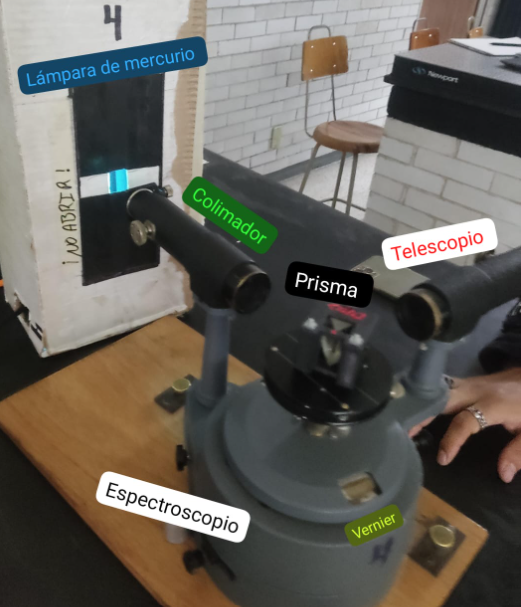
\includegraphics[width=0.4\linewidth]{arreglo 1.png}
    \caption{Arreglo experimental para la lampara de mercurio(Fotografía obtenida por Ailton Reyes)}
    \label{fig:enter-label}
\end{figure}


\subsection{Identificar de qué material está hecha una lámpara misteriosa a partir de la función obtenida de la lámpara de mercurio}

Cambiamos la lámpara de mercurio por una lámpara de un elemento misterioso sin mover el prisma. De la misma forma que con la lámpara de mercurio, alineamos el espectrómetro con la lámpara misteriosa y medimos con el vernier los ángulos de desviación para cada línea espectral, encontrando 5 (rojo, verde, cyan, azul rey y violeta).

En esta fase usamos la función polinomial de grado 3 obtenida de la lámpara de mercurio para calcular la longitud de onda de cada línea del espectro y así hacer una aproximación del posible material del que está compuesta la lámpara misteriosa.

\subsection{Inferir de qué elemento se componen 5 lámparas a partir de la observación de las líneas espectrales}
%Adivinar
Por último, se realizó un ejercicio donde se colocaron cinco lámparas de distintos elementos, y a partir únicamente de la observación de las líneas espectrales (intensidad, color y número) se tenía que Inferir de qué elemento estaba hecha cada lámpara. Para cada lámpara se tuvo un tiempo límite de observación, el cual era de cinco minutos. 

A continuación se muestran algunas líneas espectrales observadas.

\begin{figure}[h]
    \centering
    \begin{subfigure}{0.32\textwidth}
        \centering
        \includegraphics[width=\textwidth]{lineas 1.png}
    \end{subfigure}
    \hfill
    \begin{subfigure}{0.32\textwidth}
        \centering
        \includegraphics[width=\textwidth]{Lineas2.png}
    \end{subfigure}
    \hfill
    \begin{subfigure}{0.32\textwidth}
        \centering
        \includegraphics[width=\textwidth]{lineas 3.png}
    \end{subfigure}
    \caption{Ejemplos de líneas espectrales observadas(fotografías obtenidas por Andrés Gonzáles)}
    \label{fig:tres_imagenes}
\end{figure}



\section{Resultados y tratamiento de datos}

\subsection*{Alineación del espectroscopio}
Este es un paso intermedio en nuestra presentación de datos, mírese la siguiente tabla en la que obtenemos el ángulo $\theta_{incidente}$, elemento que nos servirá más adelante para calcular otras dependencias. Todas las tablas presentadas podrán encontrarse en la siguiente referencia\cite{Excel}
%%Poner las tablas nomames pedro ya ayúdame por favor no tengo ninguna incertidumbre

\begin{table}[H]
\centering
\begin{tabular}{
>{\columncolor[HTML]{D9E2F3}}c 
>{\columncolor[HTML]{FEF2CB}}c 
>{\columncolor[HTML]{E2EFD9}}c 
>{\columncolor[HTML]{D9E2F3}}c 
>{\columncolor[HTML]{FEF2CB}}c}
\cellcolor[HTML]{FFD965}$\sigma_{ap}$ {[}°{]}&
\cellcolor[HTML]{4472C4}{\color[HTML]{FFFFFF} $\theta$ {[}°{]}} & \cellcolor[HTML]{FFD965}$\Delta \theta$ {[}°{]}& \cellcolor[HTML]{92D050}$\theta_{i1}$ {[}°{]} &\cellcolor[HTML]{4472C4}{\color[HTML]{FFFFFF} $\Delta \theta_{i1}$ {[}°{]}\\
0.008 & 56& 0.13 & 62.00 & 0.07\\
\end{tabular}
\caption{Medición del ángulo de incidencia $\theta_{i1}$}
\label{tab:my-table}
\end{table}

\subsection{Medición de $n(\lambda)$ de las líneas espectrales de una lámpara de mercurio y construcción del polinomio descriptivo de longitud de onda en términos de delta}

Las longitudes de onda de la lámpara de Mercurio son ya bien conocidas por la literatura, hemos extraído las longitudes de onda de los colores presentes con mayor intensidad en su espectro de emisión de \cite{link_adicional}. \\

Utilizando el método descrito en el marco teórico \eqref{eq:nlambda}, obtenemos el índice de refracción del prisma para cada longitud de onda, véase en la siguiente tabla.

\begin{table}[H]
\centering
\begin{tabular}{
>{\columncolor[HTML]{D9E2F3}}c 
>{\columncolor[HTML]{FEF2CB}}c 
>{\columncolor[HTML]{E2EFD9}}c 
>{\columncolor[HTML]{D9E2F3}}c 
>{\columncolor[HTML]{FEF2CB}}c}
\cellcolor[HTML]{4472C4}{\color[HTML]{FFFFFF} λ {[}nm{]}} & \cellcolor[HTML]{FFD965}n experimental & \cellcolor[HTML]{92D050}$\Delta n$ &\cellcolor[HTML]{4472C4}{\color[HTML]{FFFFFF} λ {}n teórico{}}& \cellcolor[HTML]{FFD965}Diferencia \\
579 & 1.7858 &0.0022& 1.7861& 0.0003\\
577 & 1.7868 &0.0024&1.7864&0.0004 \\
546 & 1.7924 &0.0063&1.7919& 0.0005\\
492 & 1.8050 &0.0019 &1.8048& 0.0002\\
436 & 1.8254 & 0.0039&1.8252&0.0002 \\
405 & 1.8427 &0.0015 &1.8421& 0.0006
\end{tabular}
\caption{Tabla de comparativa del índice de refracción obtenido por nosotros vs lo que reporta la literatura}
\label{tab:my-table}
\end{table}

Nuestro valor está demasiado apegado a la literatura por lo que no solo es esclarecedor notar que ha sido exitoso el experimento, sino también verse que podemos aplicar este método para otras lámparas de espectros más complejos; paralelamente obtuvimos un gráfico de descripción del índice de refracción en términos de la longitud de onda. 

\begin{figure}[h]
    \centering
    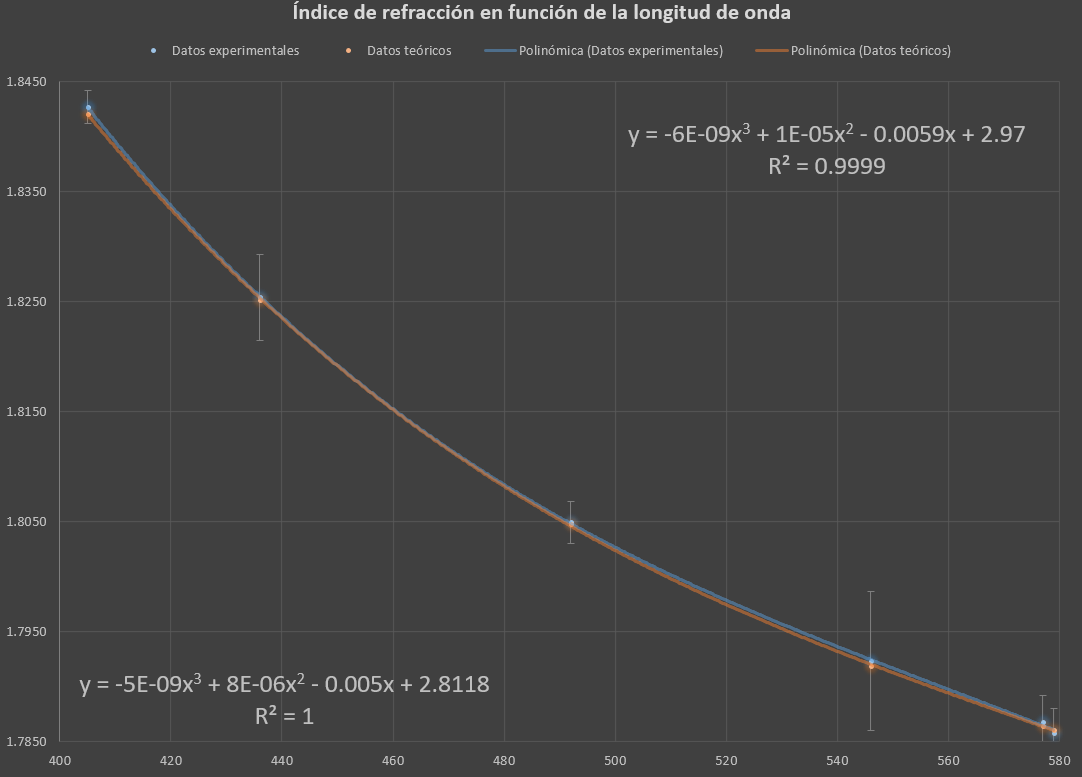
\includegraphics[width=0.5\linewidth]{indice refractivo(longitud de onda).png}
    \caption{Gráfico longitud de onda vs índice refractivo (el polinomio obtenido experimentalmente se encuentra en la zona superior derecha)}
    \label{fig:enter-label}
\end{figure}


Además, podemos graficar $\delta \quad vs \quad\lambda(\delta)$. Esto nos computa el siguiente polinomio de tercer orden que aproxima el comportamiento con coeficiente de Pearson $R^2=0.9998$.
$$\lambda(\delta) = -30051\delta^3 + 117912\delta^2 - 154732\delta + 68316$$
Esto nos será demasiado util para la siguiente fase del experimento; el gráfico de donde se obtiene el polinomio presentado se muestra a continuación:
\begin{figure}[h]
    \centering
    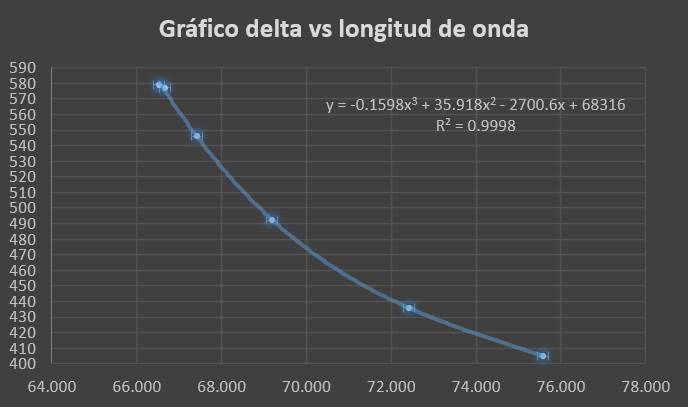
\includegraphics[width=0.5\linewidth]{Polinomio importante.png}
    \caption{Gráfico de la longitud de onda en función de delta}
    \label{fig:enter-label}
\end{figure}

\subsection{Identificar de qué material está hecha una lámpara misteriosa a partir de la función obtenida de la lámpara de mercurio}

Como se ha discutido anteriormente en el marco teórico, el polinomio obtenido en la fase anterior nos servirá para saber de qué material es esta lámpara misteriosa. Los datos obtenidos se presentan en la siguiente tabla.


%%INSERTAR LA SIGUIENTE TABLA POR FAVOR PEDRO SI LEES ESTO AYUDA, ANDREEES PONGAMOS LO DE ADIVINAR HASTA EL FINAL NO?

De aquí, al ya conocer la dependencia de la longitud de onda como una función de $\delta$, podemos simplemente evaluar en la aproximación polinomial, así es que se obtienen las siguientes longitudes de onda.

\begin{table}[H]
\centering
\begin{tabular}{
>{\columncolor[HTML]{D8D8D8}}c 
>{\columncolor[HTML]{F4B083}}c 
>{\columncolor[HTML]{D8D8D8}}c 
>{\columncolor[HTML]{D9E2F3}}c }
\cellcolor[HTML]{595959}{\color[HTML]{FFFFFF} Linea} &
  \cellcolor[HTML]{C55A11}{\color[HTML]{FFFFFF} $\delta$ {[}°{]}} &\cellcolor[HTML]{595959}{\color[HTML]{FFFFFF} $\Delta \delta$}&
  \cellcolor[HTML]{4472C4}{\color[HTML]{FFFFFF} $\lambda$ {[}nm{]}} \\
Rojo     & 65.48& 0.13 & 624.9547806 \\
Verde    & 68.08& 0.13  & 517.2633506 \\
Cyan     & 70.25&  0.13 & 462.0925047 \\
Azul Rey & 70.87& 0.13  & 450.6599968 \\
Violeta  & 72.10& 0.13  & 432.0076183
\end{tabular}
\caption{Tabla de los resultados obtenidos para longitud de onda como función del ángulo $\delta$}
\label{tab:my-table}
\end{table}

Nuevamente, con ayuda del catálogo que nos ofrece \cite{link_adicional}, hemos concluído por la intensidad de las líneas del espectro de emisión que el elemento de nuestra lámpara es cercano a Cadmio.

\subsection{Inferir de qué elemento se componen 5 lámparas a partir de la observación de las líneas espectrales}

Para esta fase del experimento, se reportaron los siguientes elementos asignados a una lampara diferente por mesa, en la siguiente tabla se muestran nuestras deducciones a partir de observar las líneas espectrales.

\begin{table}[H]
\centering
\begin{tabular}{|c|c|c|c|c|c|}
\hline
Equipo & Mesa 1 & Mesa 2 & Mesa 3 & Mesa 4 & Mesa 5 \\
\hline
VI & Nitrógeno & Kriptón & Xenón & Xenón & Argón \\
\hline
\end{tabular}
\caption{Deducción de elementos a partir de la observación del las líneas del espectro}
\end{table}

De las cuales solo acertamos en dos, en el caso de la lampara de Xenón en la mesa 4 y la lampara de Argón en la mesa 5, esto se debe a una mala interpretación de las líneas espectrales así como el tiempo límitado que se tenía para analizar cada lampara (5 min por lampara). A continuación se presenta la tabla con los elementos correctos

\begin{table}[H]
\centering
\begin{tabular}{|c|c|c|c|c|c|}
\hline
Equipo & Mesa 1 & Mesa 2 & Mesa 3 & Mesa 4 & Mesa 5 \\
\hline
VI & Neón & Nitrógeno & Kriptón & Xenón & Argón \\
\hline
\end{tabular}
\caption{Elemntos correctos}
\end{table}



\section{Conclusiones}

Los resultados obtenidos en este estudio confirman la dependencia del índice de refracción con la longitud de onda en un prisma de vidrio, validando el modelo teórico utilizado. La medición de la desviación angular permitió determinar \( n(\lambda) \) con valores experimentales en estrecha concordancia con los reportados en la literatura, con un promedio de \( n = 1.\overline{8} \pm 0.0030\). La relación funcional obtenida entre la longitud de onda y el ángulo de desviación demostró ser una herramienta eficaz para la caracterización espectral de fuentes desconocidas, permitiendo la identificación del elemento constitutivo de una lámpara de gas misteriosa. Además, el análisis cualitativo de cinco lámparas espectrales evidenció que la simple observación de las líneas espectrales es suficiente para realizar una identificación preliminar de su composición. En conjunto, estos resultados reafirman la validez de la espectroscopía de dispersión como un método preciso y versátil para el estudio de materiales ópticamente activos.



\begin{thebibliography}{9}
\bibitem{hecht2000optica} E. Hecht, \textit{Óptica}, 3ª edición, Addison Wesley, 2000.
    \bibitem{Pedrotti2018optics} F. L. Pedrotti, L. M. Pedrotti, L. S. Pedrotti, \textit{Introduction to Optics}, 3ª edición, Cambridge University Press, 2018.
    \bibitem{beiser2003concepts} A. Beiser, \textit{Concepts of Modern Physics}, 6ª edición, Mc-Graw-Hill, 2003.
    \bibitem{Polyanskiy2020refractive} M. Polyanskiy, \textit{Refractive index database}, http://refractiveindex.info/, 2008-2020.
    \bibitem{dispersionspectroscopy2025} E. Barrios B. y R. Ramírez A., \textit{Dispersión y Espectroscopía}, Óptica v.2025.

   \bibitem{link_adicional} atomic-spectra, \textit{Mercury}, recuperado de \href{https://www.atomic-spectra.net/spectrum.php?elem=Hg}{Link de la página}
       \bibitem{Excel} A. Reyes, S. Tabla Espectroscopía, Archivo Excel. 2024. Disponible en: \href{https://docs.google.com/spreadsheets/d/1C7Nac7PhHVjDRlbUn4gvEQz00NnCPn-N/edit?usp=sharing&ouid=112625838925660900694&rtpof=true&sd=true}{Enlace al documento}
\end{thebibliography}


\subsection*{Anexo}

\begin{mdframed}
\begin{equation}
    \Delta n(\lambda)= \sqrt{\left(\left|\frac{\partial n(\lambda)}{\partial \delta}\right|\Delta\delta\right)^2+\left(\left|\frac{\partial n(\lambda)}{\partial \theta_{i1}}\right|\Delta\theta_{i1}\right)^2}
\end{equation}
\end{mdframed}

Donde:

\begin{mdframed}
\begin{equation}
\frac{\partial n(\lambda)}{\partial \delta} = \frac{\cos{(\delta-\theta_{i1}+\alpha)}(\sin{(\delta-\theta_{i1}+\alpha})+\cos{(\alpha)}\sin{(\theta_{i1})})}{\sin^2{(\alpha)}\sqrt{\frac{(\sin{(\delta-\theta_{i1}+\alpha)+cos(\alpha)\sin{(\theta_{i1})}})^2}{\sin^2{\alpha}}+\sin^2{(\theta_{i1})}}}
\end{equation}
\end{mdframed}

Y :

\begin{mdframed}
\begin{equation}
\frac{\partial n(\lambda)}{\partial \theta_{i1}} = \frac{\frac{2(\cos{(\alpha)}\cos{(\theta_{i1})}-\cos{(\theta_{i1}-\delta-\alpha)})(\cos{(\alpha)}\sin{(\theta_{i1})}-\sin{(\theta_{i1}-\delta-\alpha}))}{\sin^2{(\alpha)}}+2\cos{(\theta_{i1})}\sin{(\theta_{i1})}}{2\sqrt{\frac{(cos(\alpha)\sin{(\theta_{i1})}-\sin{(\delta-\theta_{i1}-\alpha)})^2}{\sin^2{\alpha}}+\sin^2{(\theta_{i1})}}}
\end{equation}
\end{mdframed}

\begin{mdframed}
\begin{equation}
  \Delta\vartheta_i[rad] = \Delta\vartheta_i \frac{\pi}{180^{\circ}} 
\end{equation}
\end{mdframed}



\end{document}